\section{Спектральный анализ}
Спектральный анализ - это один из методов обработки сигналов, который позволяет охарактеризовать частотный состав измеряемого сигнала.
Методы статистики играют важную роль в спектральном анализе, поскольку сигналы, как правило, имеют шумовой или случайный характер. Если бы
основные статистические характеристики сигнала были известны точно или же их можно было бы без ошибк определить на конечном интервале этого
сигнала, то спектральный анализ представлял бы собой отрасль точной науки. В действительноти по одному-единственному отрезку сигнала можно
получить только некоторую оценку его спектра. Практика спектрального анализа после 1880-х гг. постепенно стала превращаеться в некое ремесло
достаточно субъективного характера, которое на ряду с использованием научного подхода требовало также определенного уровня эмпирического
искусства \cite{marpl_book}.

Математические основы современных методов спектрального оценивания берут свое начало в XVII веке в работах И. Ньютона, который установил, что
солнечный свет, прошедший через стеклянную призму, разлагается на многоцветную полосу. В которой каждому цвету соответствует своя длинна волны.

\subsection{Применение нормального уравнения Юла-Уолкера}
В 1927 г. Дж. Юл предложил существенно новый метод спектрального анализа. Для отыскаяния одной-двух переодичностей в исследуемых данных Юл
прибег к моделированию временного ряда, основанному на линейном регрессионном анализе. Юла интересовала главным образом более высокая точность
определения основной периодичности в ряде чисел солнечных пятен и отыскания в нем дополнительных периодичностей \cite{marpl_book}.
Используя простое тригонометрическое тождество:
\begin{center}
\begin{equation}
	\label{eq:yule_trigonometric}
	\sin(kx)=2\cos(x)\sin([k-1]x)-sin([k-2]x)
\end{equation}
\end{center}
Используя подстановки и обобщая формулу (весь ход обобщения описан в \cite{marpl_book}) можно получить:
\begin{center}
\begin{equation}
	\label{eq:yule_raznost}
	u(k) = b(1)u(k-1) + b(2)u(k-2) + \epsilon (k)
\end{equation}
\end{center}
Здесь ${u(k) = \sin (2\pi fkT)}$ - гармоническая составляющая, ${T}$ - интервал отсчетов, ${f}$ - частота гармоник, а
${b(1)}$ и ${b(2)}$ принимают произвольные значения. Как легко увидеть, уравнение \ref{eq:yule_raznost} представляет собой АР уравнение, и это был
первый случай когда АР по методу наименьших квадратор применялась для целей спектроанализа. Решением уравнения \ref{eq:yule_raznost}
является затухающая синусойда.

АР модель предсказания отсчета может быть описана как взвешенная сумма ${P}$ предыдущих отсчетов сигнала:
\begin{center}
\begin{equation}
	\label{eq:lpc_forecast}
	\hat{x(m)} = \sum \limits_{i=1}^P a_k x(m-k),
\end{equation}
\end{center}
Где ${\hat{x(m)}}$ - оценка ${x(m)}$ в момент времени ${m}$, а ${a_k}$ - коэффициенты АР модели.

Оценка ошибки ${e(m)}$ может быть представлена как:
\begin{center}
\begin{equation}
	\label{eq:lpc_error}
	e(m) = x(m) - \hat{x(m)} = x(m) - \sum \limits_{i=1}^P a_k x(m-k),
\end{equation}
\end{center}

????? Наилучшие оценки коэффициентов ${a_k}$ могут быть получены минимизацией среднеквадратичной ошибки уравнения
\ref{eq:lpc_error}:
\begin{center}
\begin{eqnarray}
	\label{eq:lpc_lms}
		E[e^2(m)]	& = & E[(x(m) - \sum \limits_{i=1}^P a_k x(m-k))^2] =\nonumber \\
				& = & E[x^2(m)] - \nonumber \\
				& &  - 2\sum \limits_{i=1}^P a_k E[x(m-k)x(m)] + \nonumber \\
				& &  + \sum \limits_{i=1}^P a_k \sum \limits_{j=1}^P a_j E[x(m-k)x(m-j)] = \nonumber \\
				& = & r_{xx}(0) - 2r^T_{xx}a + a^T R_{xx}a
\end{eqnarray}
\end{center}

\subsubsection{Использование АР для детектирования ШПС}
Известно, что АР подход широко применяется в детектировании и кодировании голоса и видео, в восстановлении сигналов и т.д.
Специфичной для детектирования ШПС является необходимость определения точной фазы ПСП
для работы с сигналом. Так же при обработке ШПС от нескольких источников с разными ПСП необходимо учитывать, что оценка спектра будет смещенной
и требуется его корректировка.

\paragraph{Детектирование ШПС от одного источника}

Рассмотрим применение данного подхода для детектирования одного сигнала ШПС. Схема алгоритма представлена на рисунке \ref{pic:lpc_basic}.
\begin{figure}[H]
	\center\scalebox{0.8}{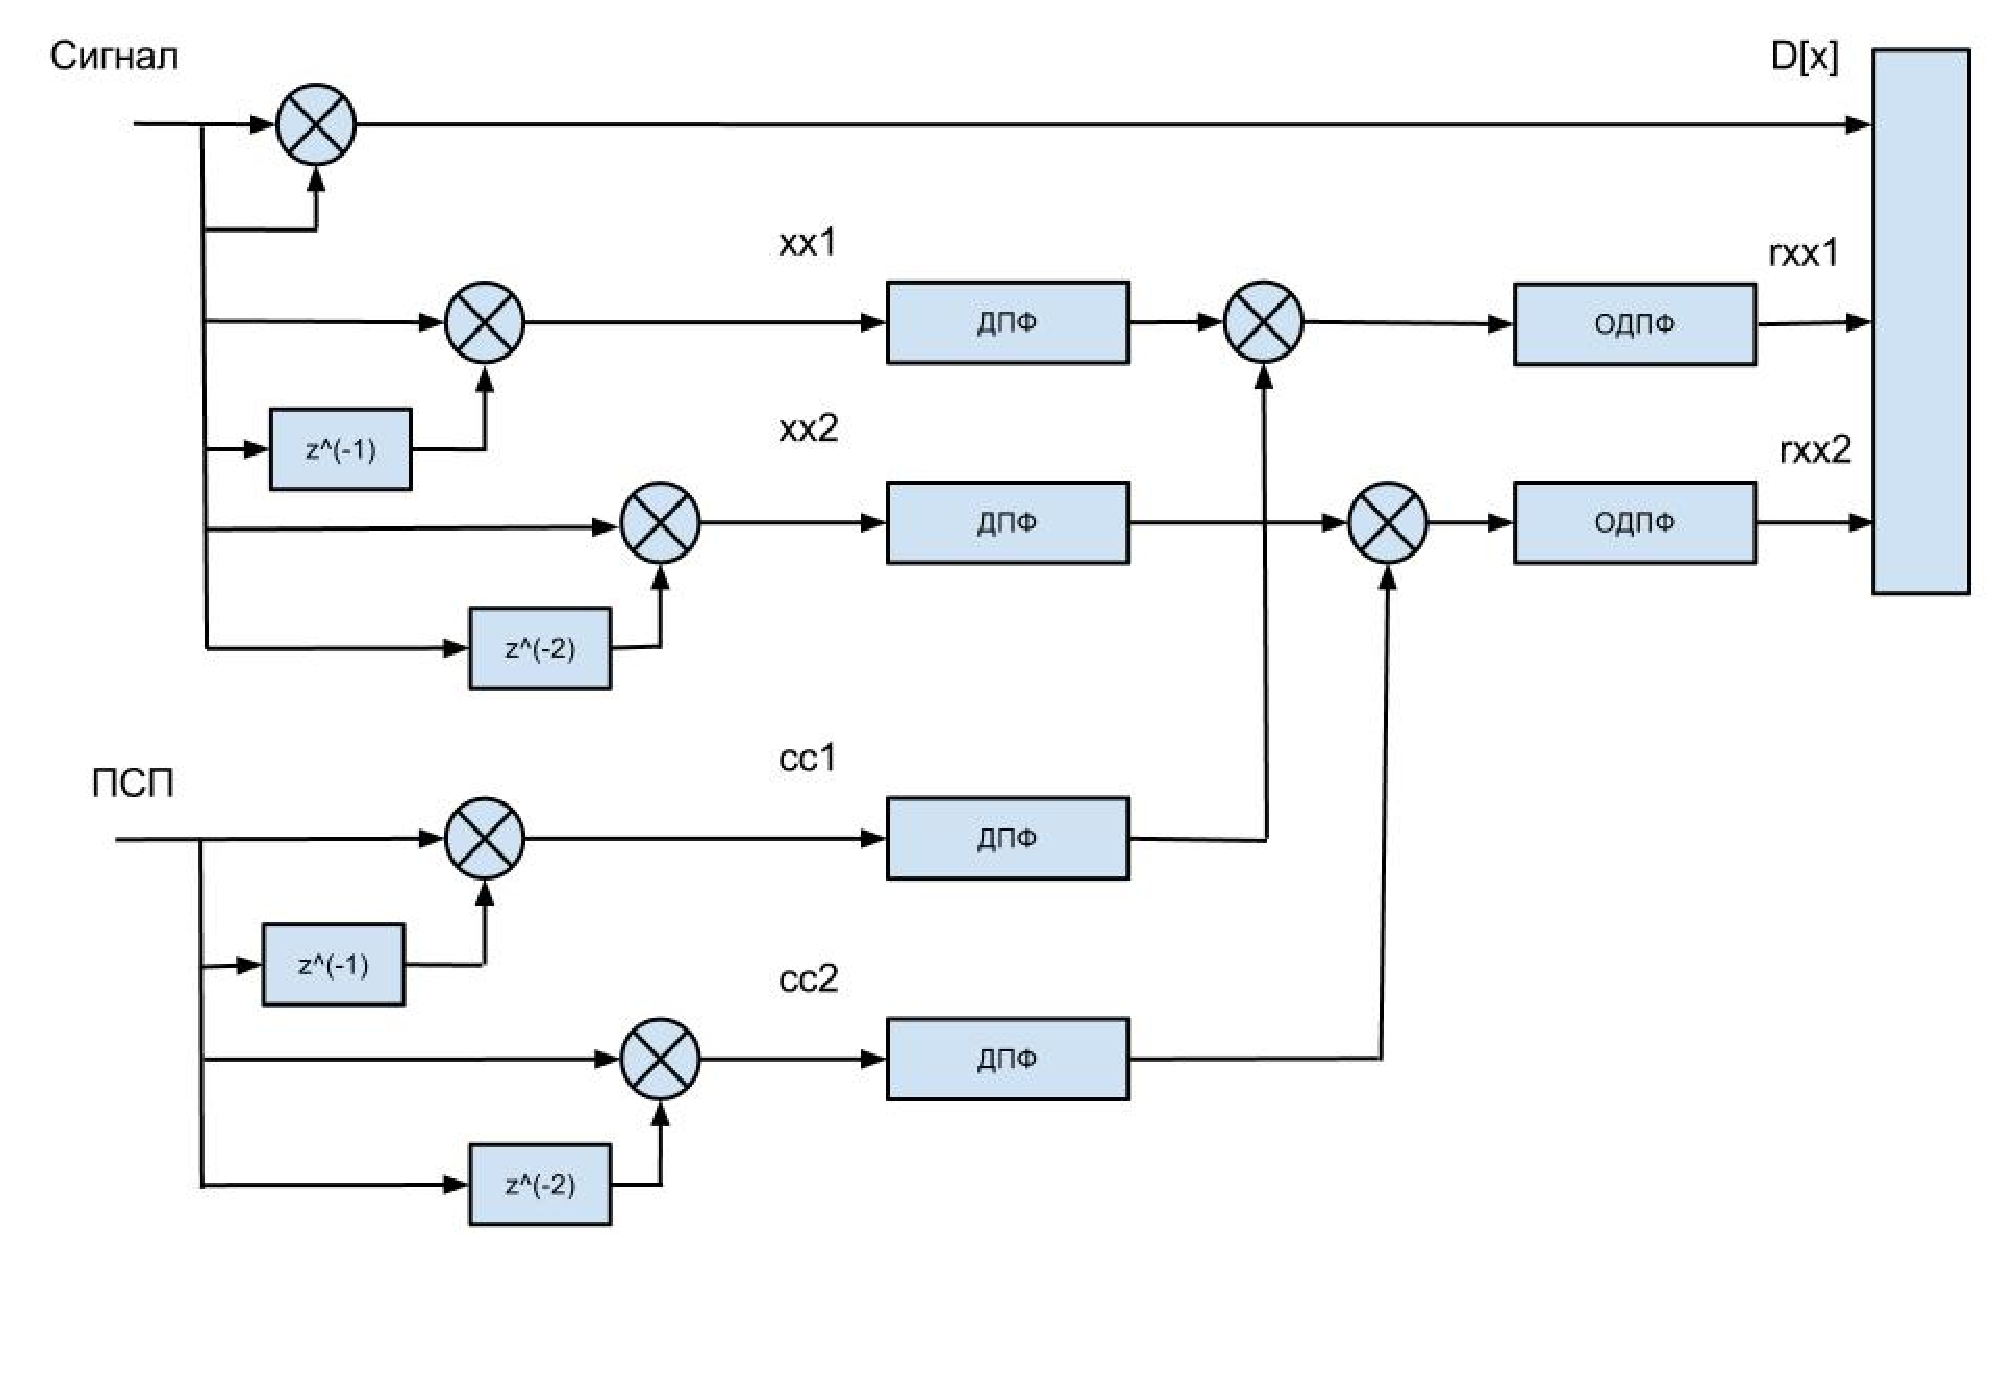
\includegraphics[width=1\linewidth]{lpc.eps}}
	\caption{Общая схема применения АР модели для детектирования ШПС сигнала}
	\label{pic:lpc_basic}
\end{figure}
Так как нам необходимо подобрать фазу ПСП мы пользуемся БПФ для отыскания всех позиций кода (глава \ref{sec1_fft}).

\begin{figure}[H]
	\center\scalebox{1}{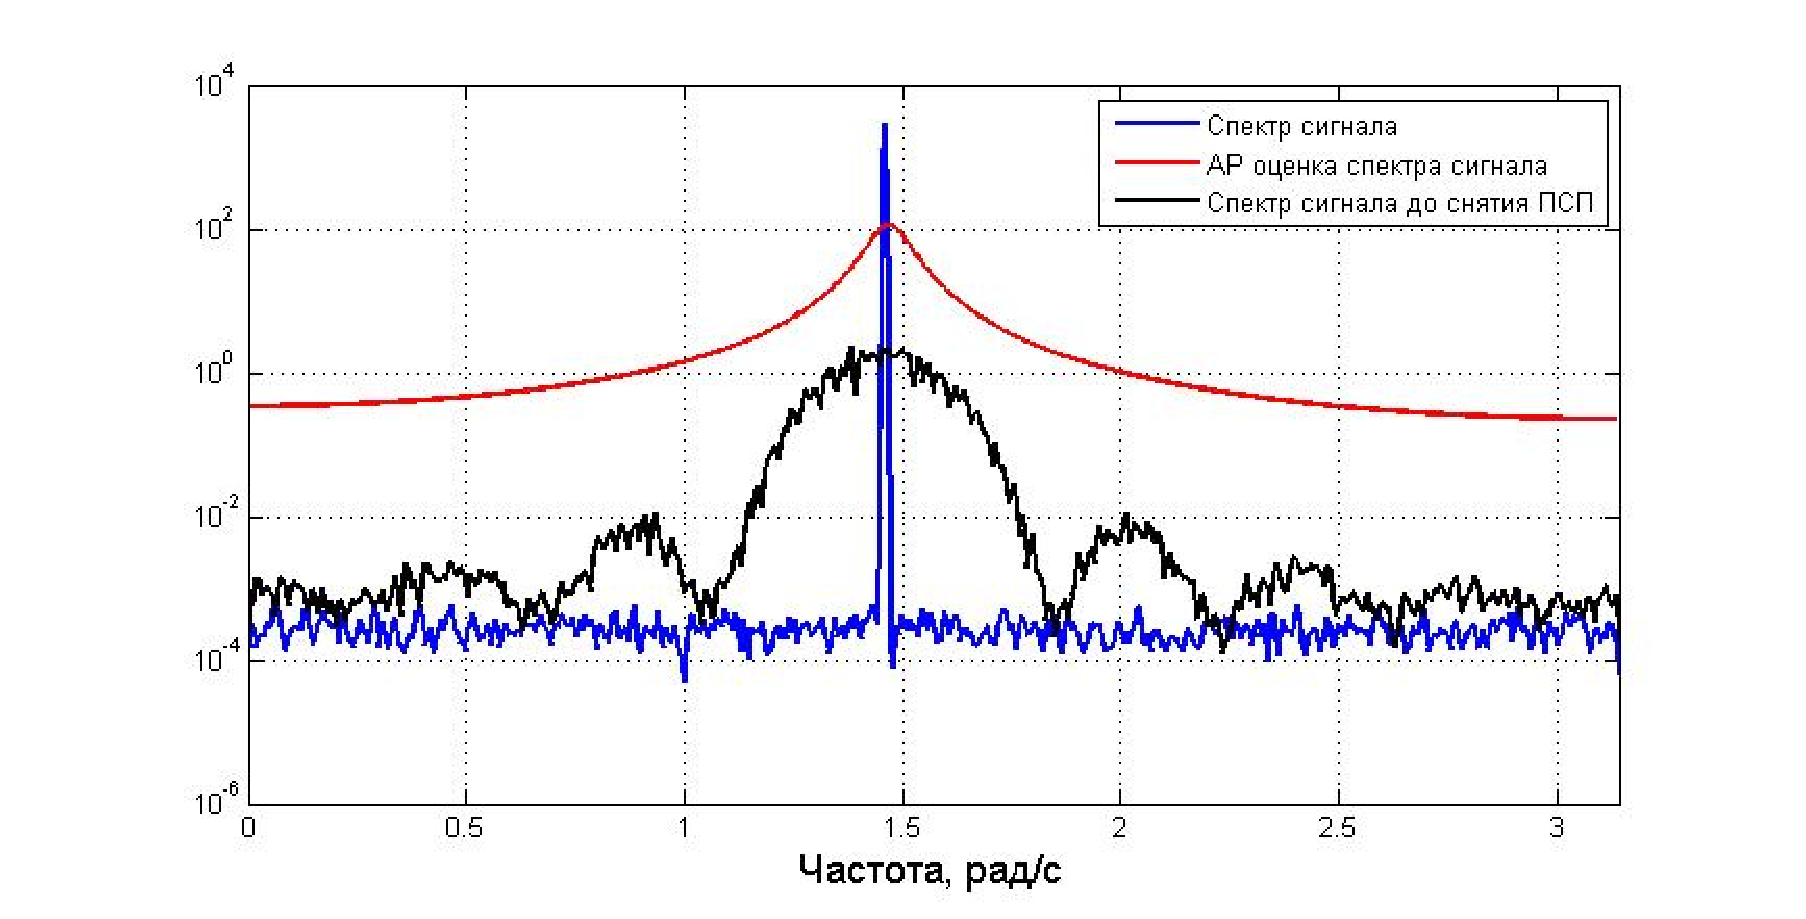
\includegraphics[width=1\linewidth]{lpc_1sat.eps}}
	\caption{Общая схема применения АР модели для детектирования ШПС сигнала}
	\label{pic:lpc_1sat}
\end{figure}

\newpage
